\documentclass[9pt,landscape]{article}

\usepackage{multicol}
\usepackage{amsmath}
\usepackage{algorithm}
\usepackage{algpseudocode}

\usepackage{amssymb}
\usepackage{amsthm}
\usepackage{amsmath}
\usepackage{fontspec,xunicode,xltxtra}
\usepackage{titlesec}
\usepackage{indentfirst}
\usepackage{xeCJK}
\usepackage{fancyhdr}
\usepackage{graphicx}
\usepackage{listings}
\usepackage{printlen}
\usepackage{ifthen}
\usepackage[savepos]{zref}
\usepackage{multicol}
\usepackage{sectsty}
\usepackage{xcolor}
\usepackage[framemethod=tikz]{mdframed}
\usepackage{hyperref}

\usepackage[letterpaper]{geometry}
\geometry{headheight=2.6cm,headsep=3mm,footskip=13mm}
\geometry{top=2cm,bottom=2cm,left=2cm,right=2cm}


\setCJKmainfont[BoldFont={SimHei}]{SimSun}
\newfontfamily{\monotype}{Consolas}
%\newcommand{\monotype}{\tt}

\pagestyle{fancy}

\fancyhead[L]{CS161 Cheat Sheet}
\fancyhead[C]{MIDTERM}
\fancyhead[R]{Summer 2024}

\setlength{\parindent}{0em}

% settings for listings
\lstset {
  basicstyle = \small\monotype,
  language = C++,
  tabsize = 2,
  breaklines = true,
  breakindent = 1.1em,
%  numbers=right,
  stringstyle=\monotype,
  numberstyle=\footnotesize\ttfamily,
%  firstnumber=last,
  basewidth={0.5em, 0.4em},
  frame=single
}

\usepackage{titlesec}

% Adjust spacing for section
\titlespacing*{\section}{0pt}{1ex plus 0.5ex minus .2ex}{1ex plus .2ex}

% Adjust spacing for subsection
\titlespacing*{\subsection}{0pt}{1ex plus 0.5ex minus .2ex}{1ex plus .2ex}

% Adjust spacing for subsubsection
\titlespacing*{\subsubsection}{0pt}{1ex plus 0.5ex minus .2ex}{1ex plus .2ex}

\usepackage{enumitem}
\setlist[enumerate]{itemsep=0pt, parsep=0pt, topsep=0pt}

% an amazing script
% converts an line-number to arbitrary string
\let\othelstnumber=\thelstnumber
\def\createlinenumber#1#2{
    \edef\thelstnumber{%
        \unexpanded{%
            \ifnum#1=\value{lstnumber}\relax
             \tt #2%
            \else}%
        \expandafter\unexpanded\expandafter{\thelstnumber\othelstnumber\fi}%
    }
    \ifx\othelstnumber=\relax\else
      \let\othelstnumber\relax
    \fi
}

\usepackage{enumitem}

\setlist[itemize]{itemsep=0pt, parsep=0pt, topsep=0pt}
 % formatting template

\begin{document}

\begin{multicols}{2}

\columnseprule=0.25pt

\section{Security Principles}

\begin{enumerate}
    \item \textbf{Know your threat model}: 谁会来攻击你,为什么要攻击你。Threat Model 指的就是对攻击者建立一个合适的模型(比如他们有多少资源,他们的动机)。\emph{You often just need to have ``good enough'' defense to make attackers turn somewhere else.}
    \item \textbf{Consider Human Factors}: 考虑用户习惯,别让用户太麻烦。
    \item \textbf{Security is economics}: 搞 security 需要米,所以要考虑你保护的是啥。
    \item \textbf{Detect if You Can't Prevent}:
        \begin{itemize}
            \item \textbf{Deterrence}: Stop the attack before it happens.
            \item \textbf{Prevention}: Stop the attack as it happens.
            \item \textbf{Detection}: Learn that there was an attack (after it happened).
            \item \textbf{Response}: Do something about the attack (after it happened). 对于 response,需要做的事 Mitigation and Recovery,就是比如在发现勒索软件的时候赶紧进行文件备份和转移。
        \end{itemize}
    \item \textbf{Defense in depth}: 多层防御,但是要考虑成本。
    \item \textbf{Least Privilege}: 然鹅其实现在的操作系统做的都很遭糕。
    \item \textbf{Ensure complete mediation}: You should check \emph{every} access to \emph{every} object. 课上提出了一个叫做 \emph{Reference Monitor} 的概念,就是一个任何 access 操作都必须经过的结点,比如说 network firewall。用这种方法来保证每个 access 都被检查过。
    \item \textbf{Separation of Responsibility}: 例子是原子弹发射,要两个人同时操作才行。
    \item \textbf{Shannon's Maxim}: 你不能依赖于 Security Through Obscurity,也就是通过源代码的保密性来保护系统。想到 Kerckhoff's Principle?
    \item \textbf{Use Fail-Safe Defaults}: 当系统崩溃的时候,应该让系统保持最安全的状态。比如说一些防盗门在断电的时候要自动关上。
    \item \textbf{Design in Security from the Start}
\end{enumerate}

\textbf{TCB Design Principles}:

\begin{itemize}
\item Unbypassable (or completeness)
\item Tamper-resistant (or security):不能改,必须保证 TCB 的完整性
\item Verifiable (or correctness):TCB 应该设计得越小越好(KISS principle: Keep It Simple, Stupid)
\end{itemize}

TOCTTOU Vulnerabilities

\section{Memory Safety}

\subsection{x86 Calling Convention}

\begin{enumerate}
\item Push arguments onto the stack (reverse order).
\item Push the old \texttt{EIP} onto the stack. This value becomes the \texttt{RIP}.
\item Move \texttt{EIP} to the first instruction of the function.
\item Push the old \texttt{EBP} onto the stack. This value becomes the \texttt{SFP}.
\item Move the \texttt{EBP} down to \texttt{ESP} to start a new frame.
\item Move the \texttt{ESP} down to allocate space for local vars.
\item Execute the function.
\item Move the \texttt{ESP} up to the \texttt{EBP}.
\item Pop the \texttt{SFP} and move the \texttt{EBP} to that value.
\item Pop the \texttt{RIP} and move the \texttt{EIP} to that value.
\item Remove arguments from the stack.
\end{enumerate}

\subsection{GDB}

\texttt{finish}: 相当于 step out

\texttt{info registers}

\texttt{info frame}

\texttt{disas <function\_name>}

\subsection{C}

\begin{lstlisting}
gets -> fgets
strcpy -> strncpy / strlcpy
strlen -> strnlen / memchr
\end{lstlisting}

\texttt{size\_t} 在大部分机子是 \texttt{uint32\_t}

\texttt{printf("000\%n", \&val)}: 写入 \texttt{0x00000003} 到 \texttt{\&val}

\texttt{printf("000\%hn", \&val)}: 写入 \texttt{0x0003} 到 \texttt{\&val}

在末尾写入 \texttt{"\textbackslash 0"} 的函数:\texttt{gets}, \texttt{fgets}, \texttt{strcpy}

\texttt{strncpy} 要看有没有在前 $n$ 个字符中读到 \texttt{"\textbackslash 0"}

\begin{lstlisting}
size_t fread(void *buffer, size_t size, size_t count, FILE *stream);
\end{lstlisting}

\texttt{fread} 不加 \texttt{"\textbackslash 0"}

\begin{lstlisting}
char *strncpy (char *destination, const char *source, size_t num);
\end{lstlisting}

返回 \texttt{destination}

\begin{lstlisting}
size_t strnlen(const char *s, size_t maxlen);
\end{lstlisting}

\section{Cryptography}

\subsection{Definitions}

\textit{Confidentiality} is the property that prevents adversaries from reading our private data.

\textit{Integrity} is the property that prevents adversaries from tampering with our private data.

\textit{Authenticity} is the property that lets us determine who created a given message.

\textit{Deniability}: 可否认性,这不是我说的!

Kerckhoff's Principle

Threat Models: Ciphertext-only, Chosen-plaintext, Chosen-ciphertext, Chosen plaintext-ciphertext

chosen 啥就是 Eve 可以把选择特定的啥然后 encrypt / decrypt

IND-CPA: $M_0$ 和 $M_1$ 是 Eve 给的,但必须长度相同,A 来选

To break IND-CPA, Eve must learn something other than message length

$\varepsilon\le\frac{1}{2^{80}}$ is a reasonable threshold

\subsection{One-Time Pad}

OTP 不是 IND-CPA secure 的

\subsection{Block Ciphers}

Key size ($k$) 128, 192, or 256 bits,一般用 256

Block size ($n$) 128 bits

Electronic Code Book (ECB) is deterministic

Cipher Block Chaining (CBC): Unpredictable $\mathrm{IV}$

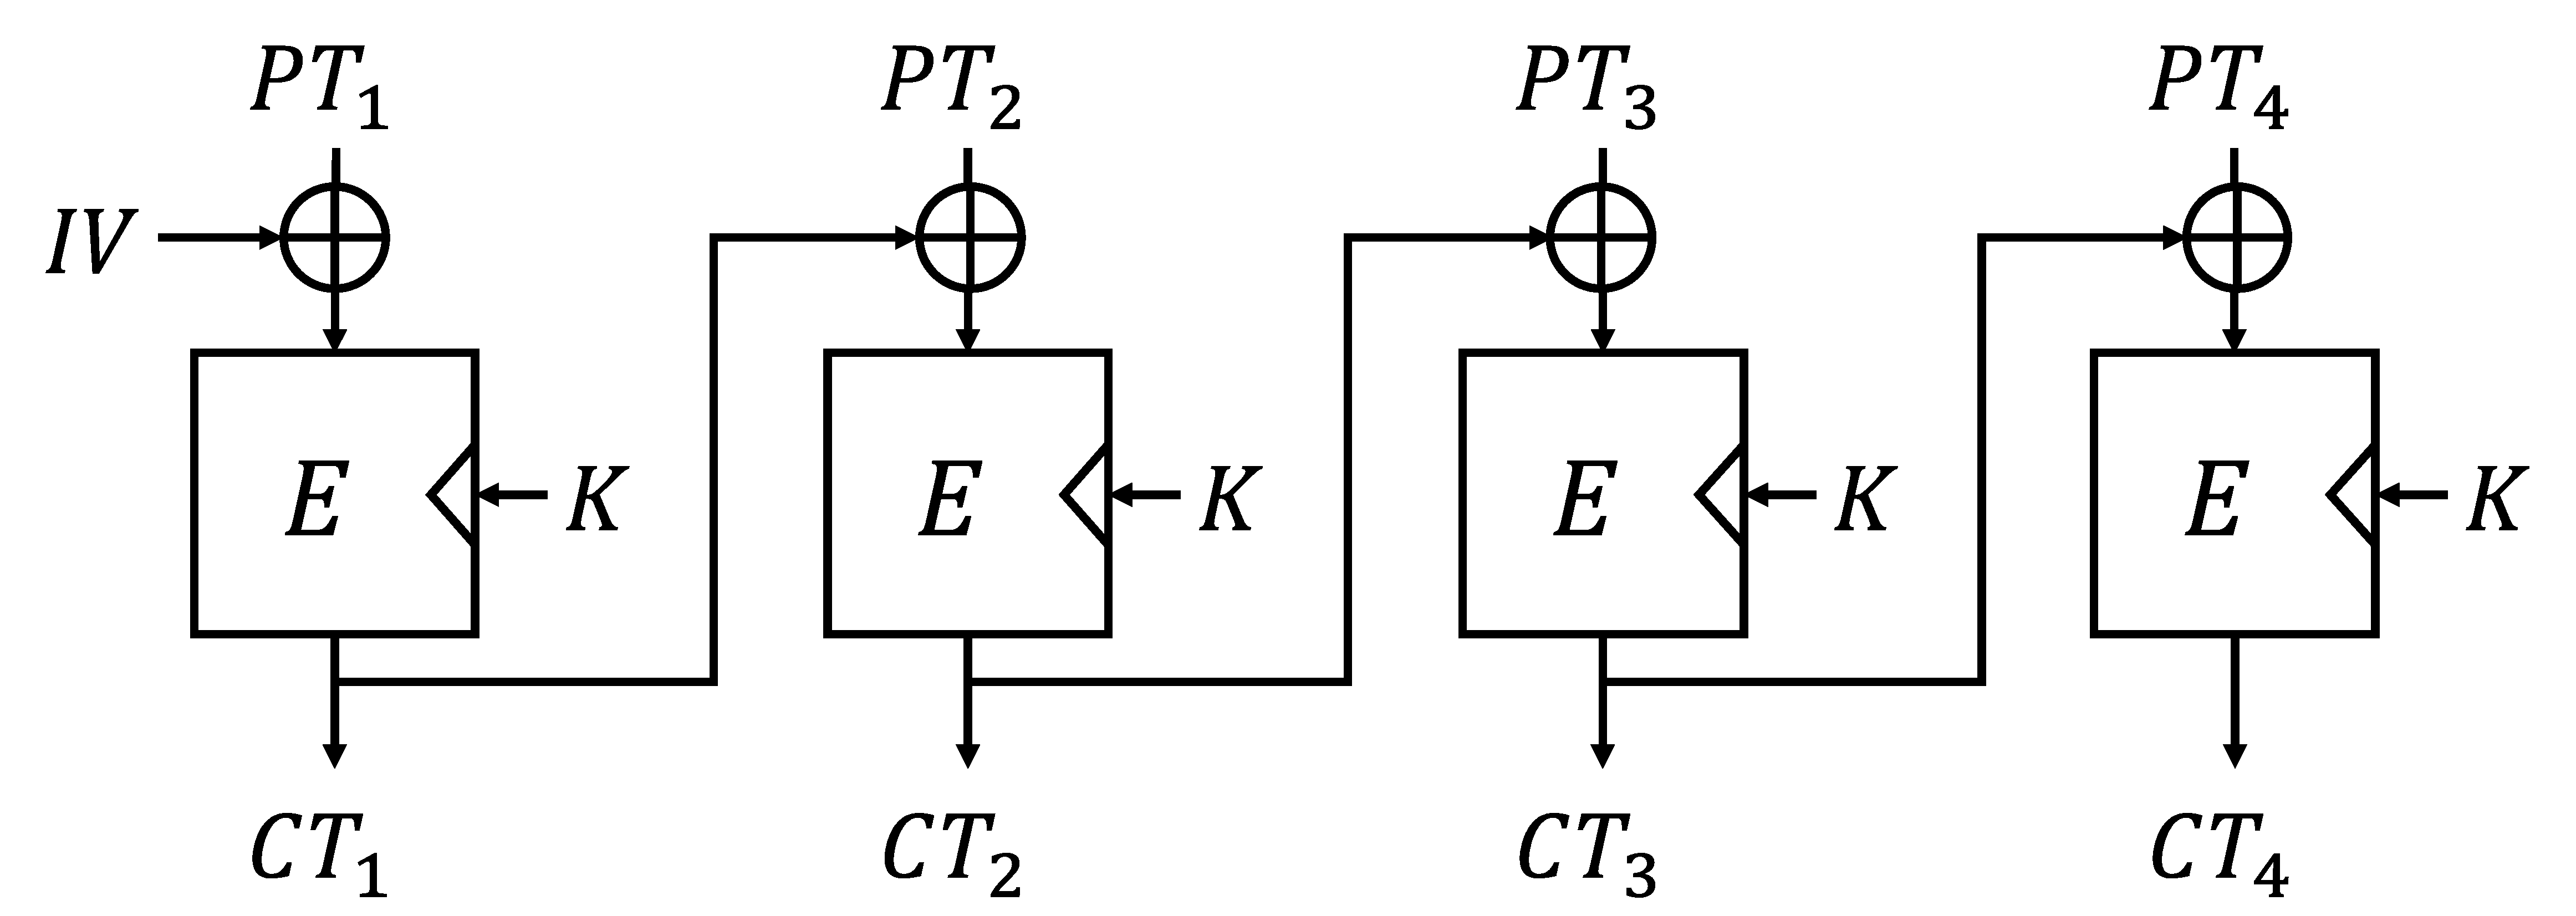
\includegraphics[width=\columnwidth]{imgs/CBC}

CTR Mode: Nonce unique

$C_i=E_k(\mathcal{N}\Vert i)\bigoplus P_i$

CFB Mode

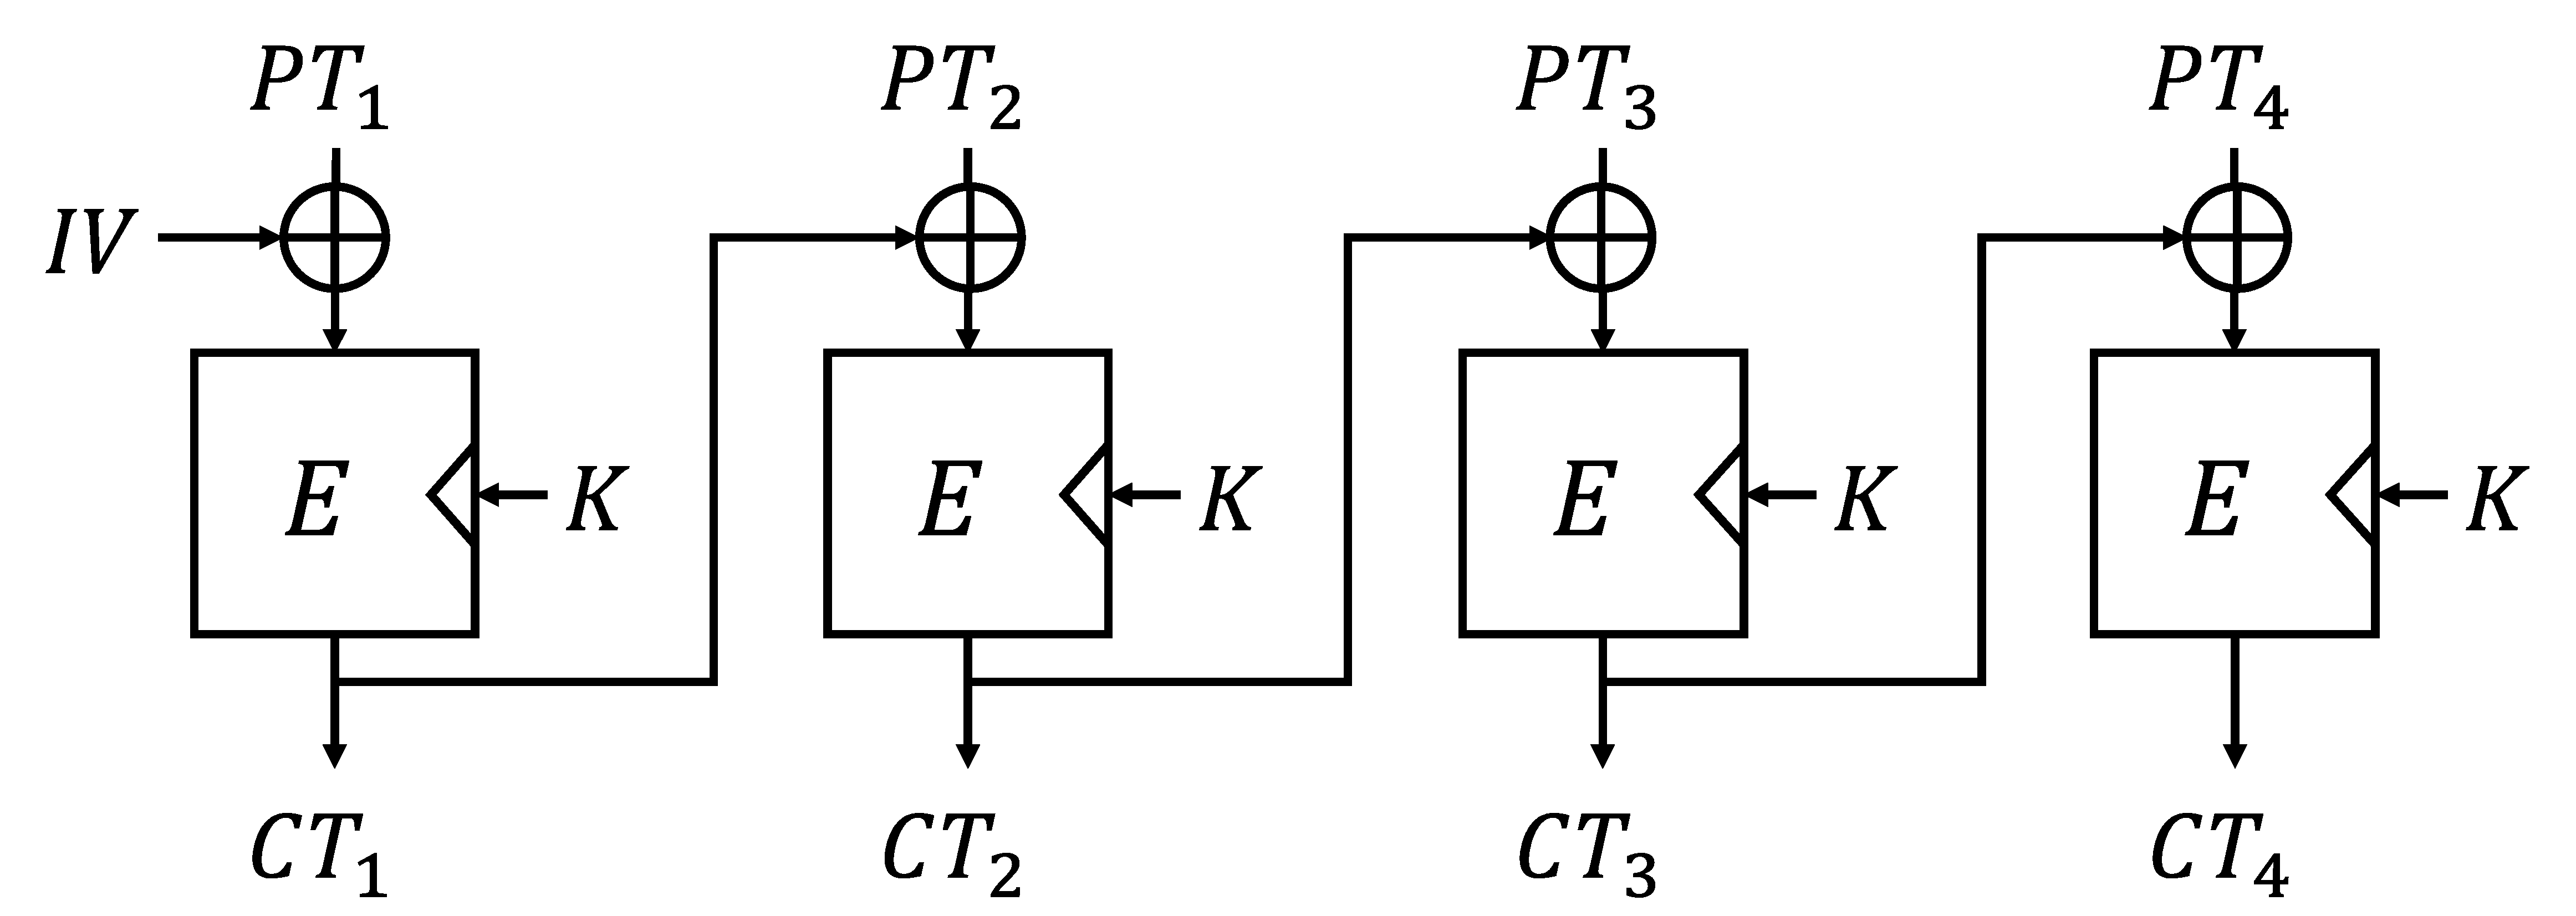
\includegraphics[width=\columnwidth]{imgs/CBC}

\subsection{Hash}

One-way-ness (``preimage resistance''): 随便给个 $y$ 很难找到 $H(x)=y$ ($H(x)=1$ 不是)

Collision Resistance, birthday attack

Random / unpredictability: 改一个就会影响很大

常见的 Hash Functions:

MD5: 128 bits output, completely broken

SHA-1: 160 bits output, completely broken in 2017

SHA-2: 256, 384, or 512 bits (sometimes labeled SHA-256, SHA-384, SHA-512). Not currently broken, but some variants are vulnerable to a length extension attack. Current standard.

SHA-3 (Keccak): 256, 384, or 512 bits. Current standard.

要注意 hash provide integrity 需要在 hash 值不被改的前提下

Length extension: 给你 $\mathcal{H}(x)$ 和 $x$ 的长度,可以构造出 $\mathcal{H}(x\Vert m)$(SHA-256)

\subsection{MACs}

Message Authentication Codes

$\mathrm{MAC}(K, M)\to T$, generate a tag

大部分 MACs 是 deterministic 的

EU-CPA: existentially unforgeable,但不要求 non-deterministic,所以不能造之前出过的数据

$\mathrm{NMAC}(K_1, K_2, M) = \mathcal{H}(K_1\Vert \mathcal{H}(K_2\Vert M))$

用两次 hash 是为了防止 length extension

$\mathrm{HMAC}(K, M)$: $K_1=K_0\bigoplus \mathrm{ipad}, K_2=K_0\bigoplus\mathrm{opad}$

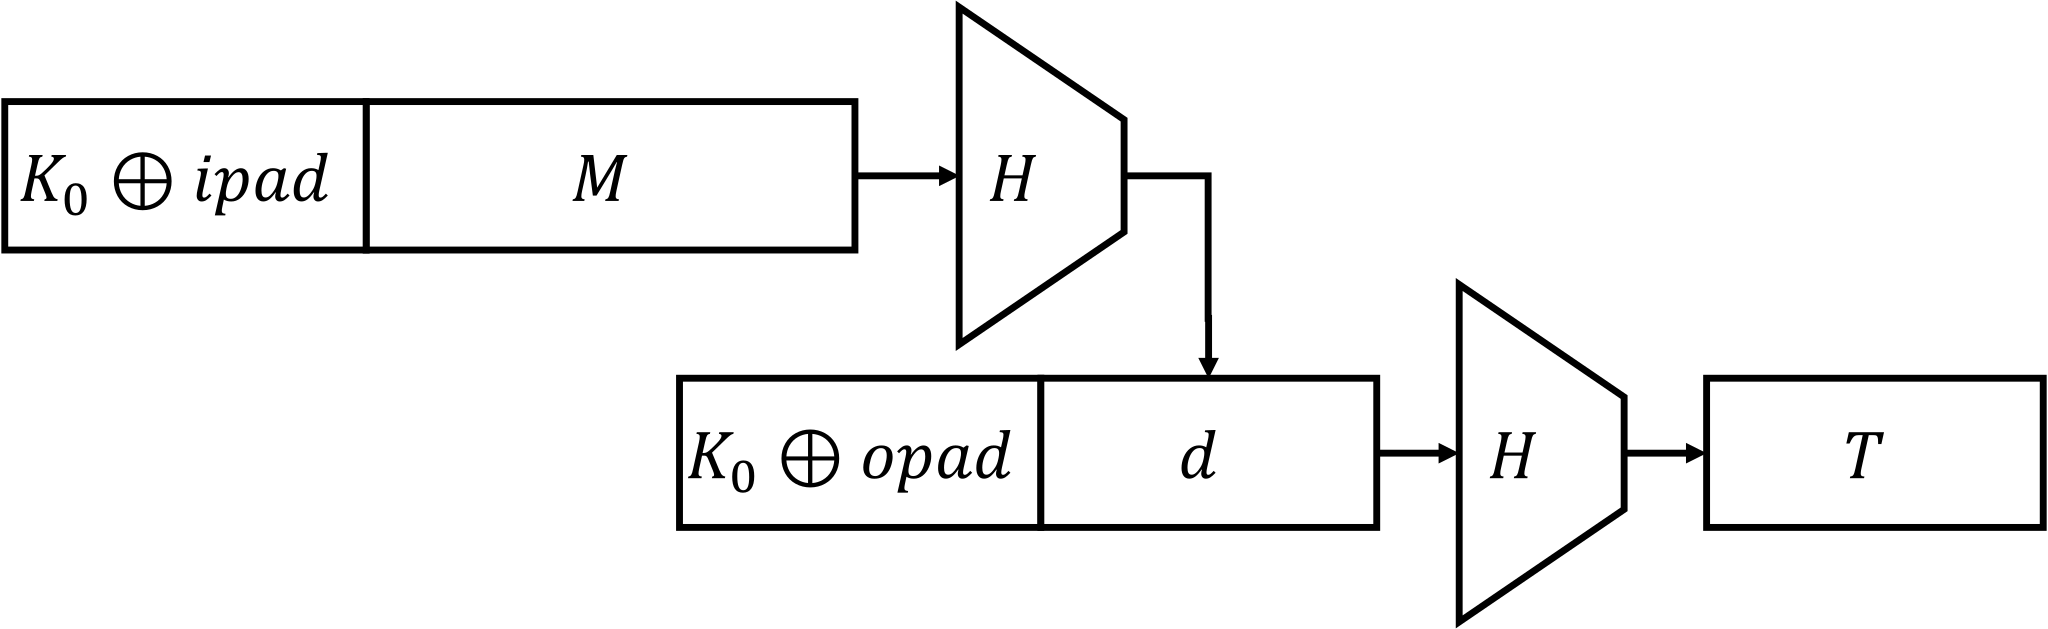
\includegraphics[width=\columnwidth]{imgs/HMAC}

$K_0$ 是 preprocess 过的 $K$,太长 hash,太短 pad 0

\texttt{ipad = 0x5c * len(k\_0)}

\texttt{opad = 0x36 * len(k\_0)}

但 HMAC 是 deterministic 的

\subsection{Authenticated Encryption}

Always use encrypt-then-MAC

$\mathrm{MAC}(K_2, \mathrm{ENC}(K_1, M))$

MAC-then-encrypt 也是对的,但是比较难写

不能 key reuse: $K_1\neq K_2$

Authenticated encryption with additional data (AEAD): 直接 provide both confidentiality and integrity over the plaintext and integrity over additional data

Galois Counter Mode (GCM): AEAD,但是比较难写难用,用错了之前 leak everything

\subsection{PRNGs}

Pseudorandom number generator, also called deterministic random bit generators (DRBGs)

3 bits of entropy = uniform, random distribution over 8 values

PRNGs are deterministic

Rollback resistance: but not required

CTR-DRBG: $\mathtt{PRNG.seed}(K\Vert\mathrm{IV})$

$\mathtt{generate}(m)=\mathrm{E}_k(\mathrm{IV}\Vert 1)\Vert\cdots\Vert\mathrm{E}_k\left(\mathrm{IV}\Vert \left\lceil\frac{m}{n}\right\rceil\right)$

HMAC-DRBG

\begin{minipage}{\linewidth}
    \begin{algorithm}[H]
    \caption{Seed Generation for HMAC-DRBG}
    \begin{algorithmic}[1]
    \State \textbf{Input:} Seed $s$
    \State $K \gets 0$
    \State $V \gets 0$
    \State $K \gets \text{HMAC}(K, V \| \mathtt{0x00} \| s)$
    \State $V \gets \text{HMAC}(K, V)$
    \State $K \gets \text{HMAC}(K, V \| \mathtt{0x01} \| s)$
    \State $V \gets \text{HMAC}(K, V)$
    \end{algorithmic}
    \end{algorithm}
\end{minipage}

Reseed: 把 seed 中的 $K, V\gets 0, 0$ 去掉

\begin{minipage}{\linewidth}
    \begin{algorithm}[H]
    \caption{Generation for HMAC-DRBG}
    \begin{algorithmic}[1]
    \State $o\gets\mathrm{EmptyString}$
    \While {len(output) $<$ n}
        \State $V \gets \mathrm{HMAC}(K, V)$
        \State $o \gets o \| V$
    \EndWhile
    \State $K \gets \mathrm{HMAC}(K, V \| \mathtt{0x00})$
    \State $V \gets \mathrm{HMAC}(K, V)$
    \State \Return $o_{1\sim n}$
    \end{algorithmic}
    \end{algorithm}
\end{minipage}

Assuming HMAC is secure, HMAC-DRBG is a secure, rollback-resistant PRNG

UUID: use PRNGs

\subsection{Stream Ciphers}

AES-CTR is a type of stream cipher

不要用同一个 key encrypt 太多 PT:如果 key 是 $n$ bits long,最多只能 encrypt $2^{\frac{n}{2}}$ 个 blocks

\subsection{DHE}

DHE is an active protocol

DHE does not provide authentication

ECDH: Elliptic-curve Diffie-Hellman

\subsection{Public-Key Encryption}

$PK$: Public key

$SK$: Private key

\subsubsection{ElGamal}

Bob 生成 SK $b$ 和 PK $B=g^b$

A 生成随机 PK $r$ 和 PK $R=g^r$

$C = (R, M\times B^r)$

$P = C_2\times C_1^{-b}$

\subsubsection{RSA}

PK: $N = pq, e$

SK: $d \equiv e^{-1}\pmod{(p-1)(q-1)}$

$e$ 是 $(p-1)(q-1)$ 的 coprime

$\mathrm{Enc}(e, N, M) = M^e \mathrm{\ mod\ }N$

$\mathrm{Dec}(d, C) = C^d\mathrm{\ mod\ }N$

$e$ is usually small (about $16$ bits) and often constant ($3, 17, 65537$)

Optimal asymmetric encryption padding (OAEP): add randomness

Hybrid Encryption: 先用 asymmetric 传密钥再用 symmetric 传数据

\subsection{Digital Signatures}

$S = {\mathcal{H}(M)}^d\mathrm{\ mod\ }N$

Verify: check $S^e\equiv\mathcal{H}$

\end{multicols}

\end{document}
